\section{Coupled System}

\subsection{Testing}
Before we investigate the effects of increasing the coupling strength between the two systems, we verify that if the hopping amplitude $v_c = 0$, the spectra on the individual sites remain unchanged. For the coupled system, calculating the Lehmann spectrum is no longer an option as memory becomes a limiting factor, instead we resort to using the Green's function method.

\medskip
As can be seen when comparing Fig. \ref{fig:coupled_vc_0} with the spectra in Fig. \ref{fig:spectrum_engineering} and Fig. \ref{fig:isolated_benzene}, this is indeed the case. The slight variations being due to a difference in parameters used to perform the Fourier transformation.

\begin{figure}[!hbt]
    \centering
    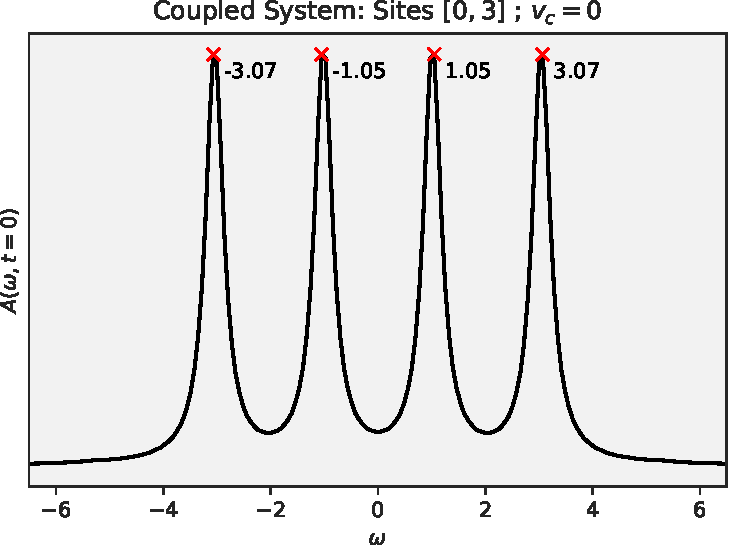
\includegraphics[width=0.49\textwidth]{graph/coupled_QD_vc_0.pdf}
    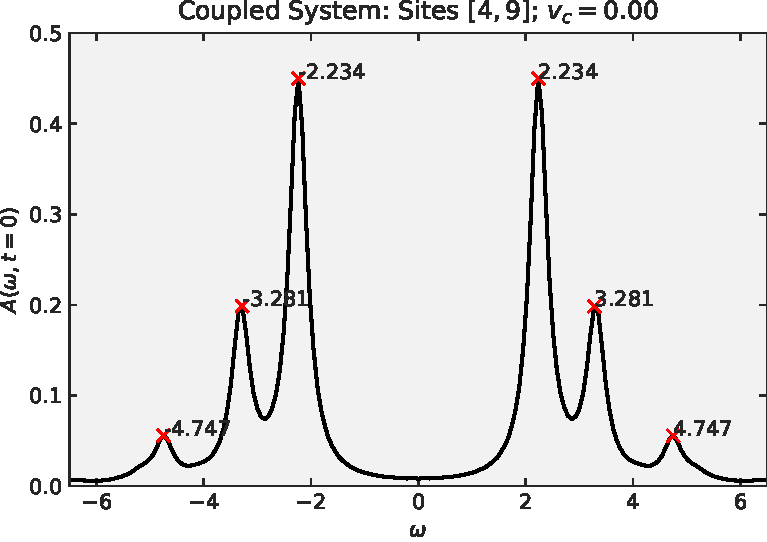
\includegraphics[width=0.49\textwidth]{graph/coupled_benzene_vc_0.pdf}
    \caption{Spectral function of all the sites of the coupled system with the coupling parameter turned off, $v_c = 0$. These spectra should be identical to those in Fig. \ref{fig:spectrum_engineering} and Fig. \ref{fig:isolated_benzene}}
    \label{fig:coupled_vc_0}
\end{figure}

\subsection{Dependence of the spectrum on the coupling strength}
Fig. \ref{fig:spectrum_vc_sweep_QD} and Fig. \ref{fig:spectrum_vc_sweep_benzene} show how the spectrum changes on each site, as the coupling strength $v_c$ between the QD and the benzene ring is increased. Notice that the symmetry of the geometry is preserved, as all QD sites show the same spectra. The benzene site pairs 5, 9 and 6, 8 also each share identical spectra since they are symmetric about site 4, which is coupled to the QD. \color{red} I can not really do more than describe how the graphs look, as I do not feel that I have a deep enough understanding in order to interpret and draw conclusions form these graphs\color{black}

\begin{figure}[!hbt]
    \centering
    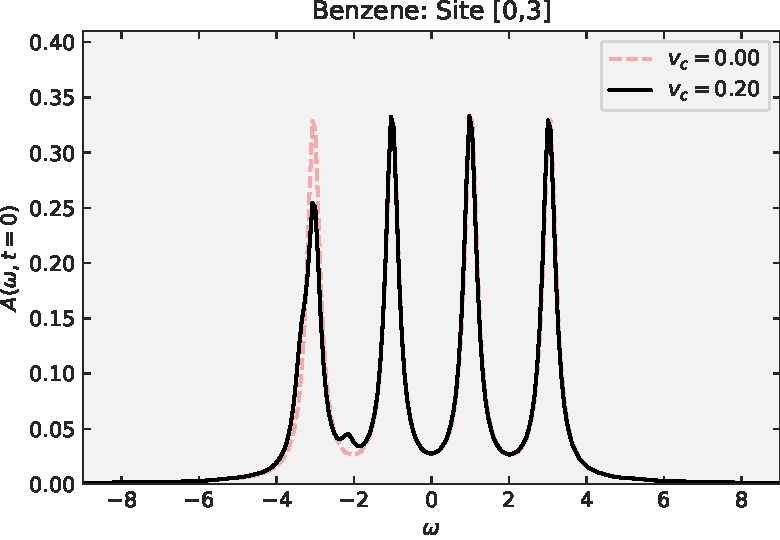
\includegraphics[width=0.49\textwidth]{graph/spectrum_vc_sweep/QD_All_020.pdf}
    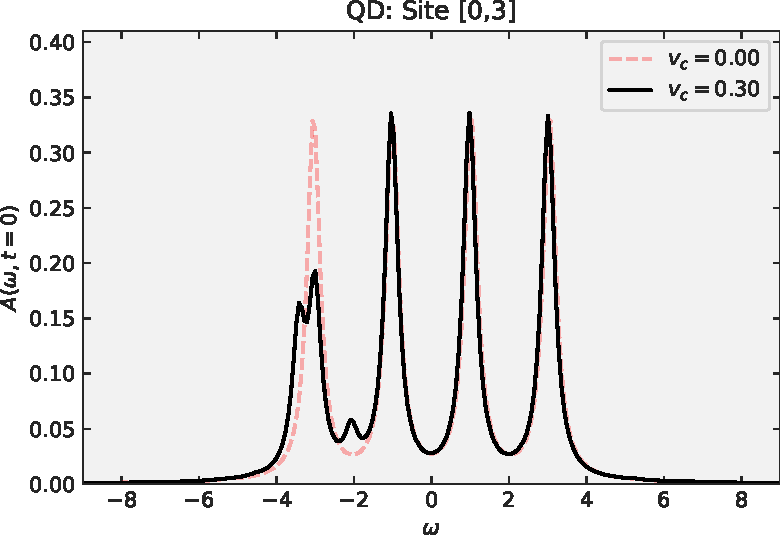
\includegraphics[width=0.49\textwidth]{graph/spectrum_vc_sweep/QD_All_030.pdf}
    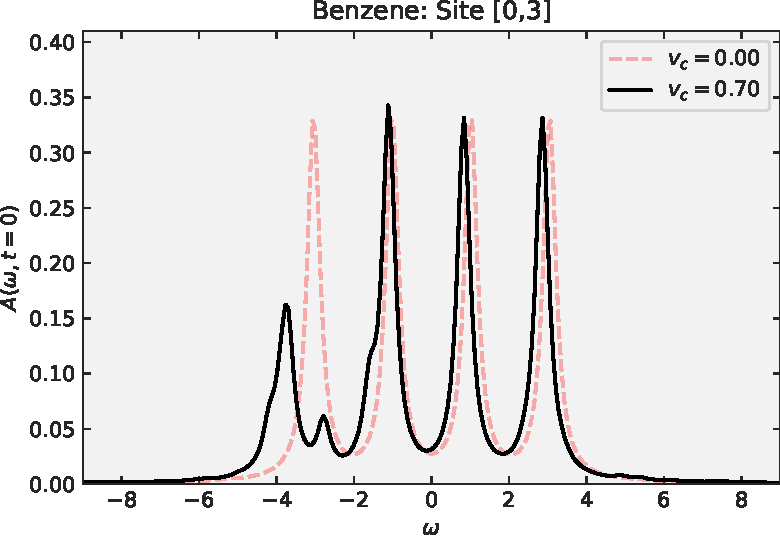
\includegraphics[width=0.49\textwidth]{graph/spectrum_vc_sweep/QD_All_070.pdf}
    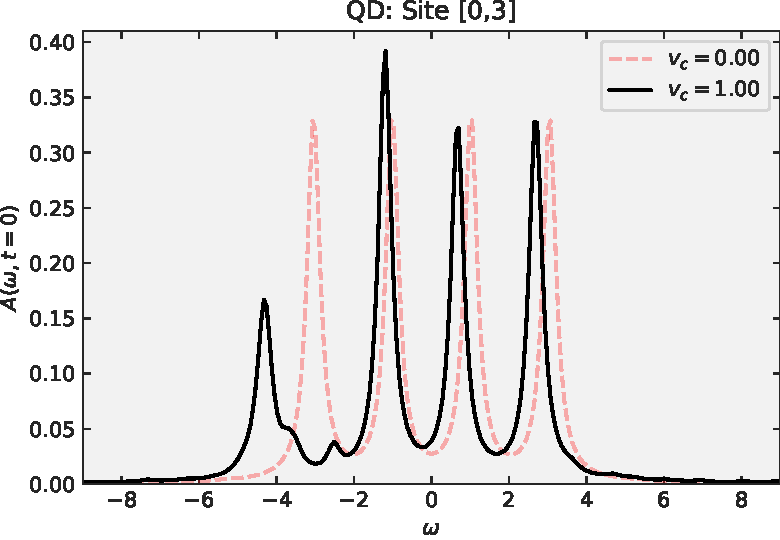
\includegraphics[width=0.49\textwidth]{graph/spectrum_vc_sweep/QD_All_100.pdf}
    \caption{Changes in the spectral function of the QD with increasing coupling $v_c$ to the benzene ring}
    \label{fig:spectrum_vc_sweep_QD}
\end{figure}

\begin{figure}[!hbt]
    \centering
    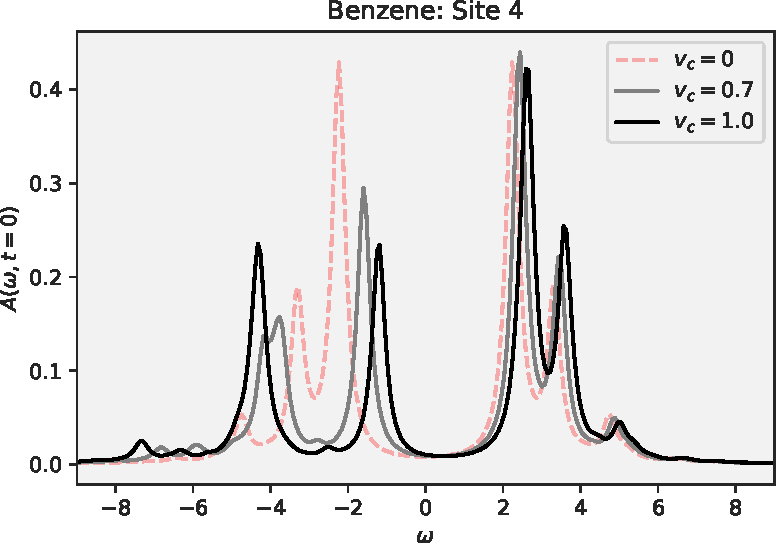
\includegraphics[width=0.49\textwidth]{graph/spectrum_vc_sweep/Benz_4_07_10.pdf}
    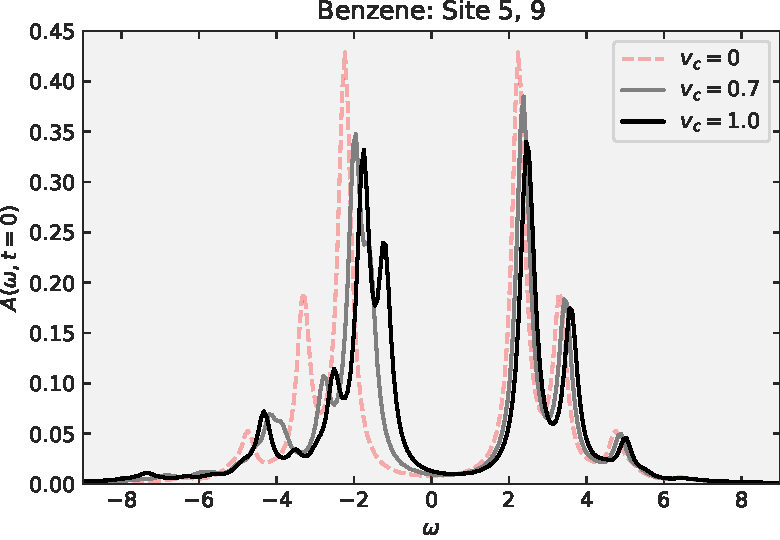
\includegraphics[width=0.49\textwidth]{graph/spectrum_vc_sweep/Benz_59_07_10.pdf}
    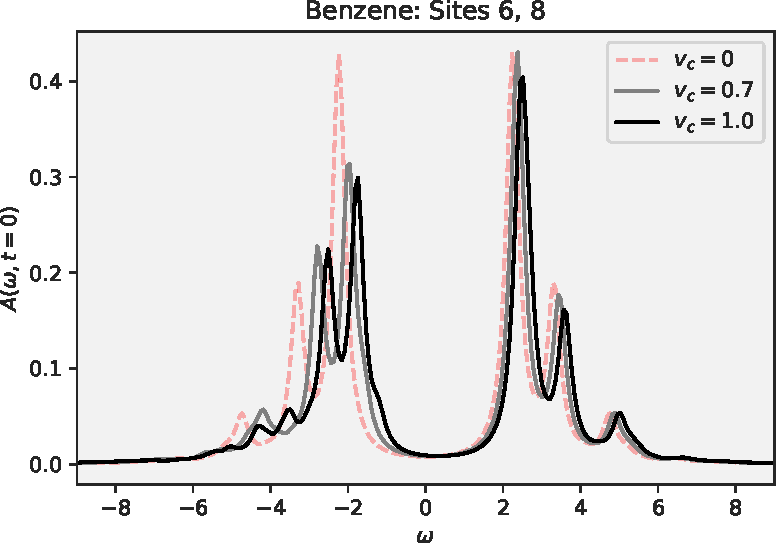
\includegraphics[width=0.49\textwidth]{graph/spectrum_vc_sweep/Benz_68_07_10.pdf}
    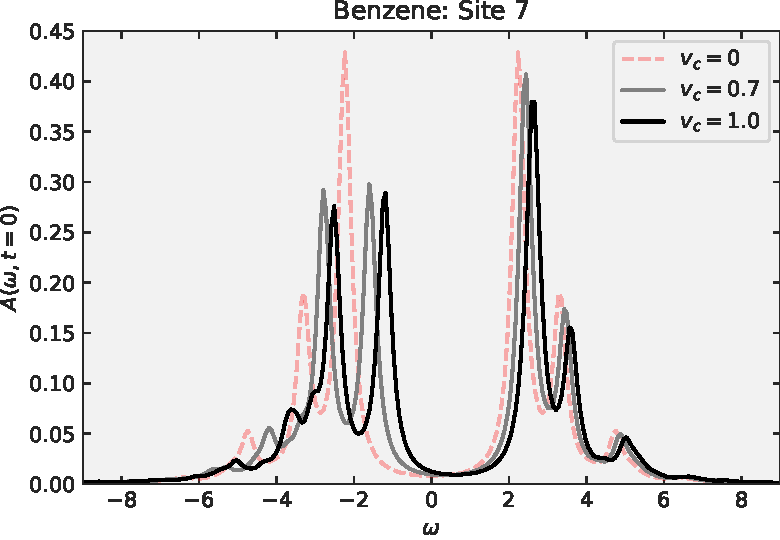
\includegraphics[width=0.49\textwidth]{graph/spectrum_vc_sweep/Benz_7_07_10.pdf}
    \caption{Changes in the spectral function of the benzene ring with increasing coupling $v_c$ to the QD}
    \label{fig:spectrum_vc_sweep_benzene}
\end{figure}

\subsection{Interaction energy and impact ionisation}
Ideally we would like to to investigate the changes in interaction energy on the QD and on the benzene ring separately, however, because all the calculations happen in the state basis, and the interaction energy depends on multiple sites, calculating the observable on a particular set of sites is non-trivial. In the state basis each basis vector is a state of the entire system and thus all sites are always involved, making it impossible to separate which sites the contributions come from without a change of basis. Performing a transformation into the site basis is outside the scope of this work, thus we will only be looking at the interaction energy of the system as a whole.
\medskip

Fig. \ref{fig:interaction_energy_omega} shows the interaction energy $\braket{\hat{E}_{\rm int}}$ for a light pulse energy $\omega = 2$, and $\omega=4$. Once without coupling of the QD to benzene ($v_c=0$) and once with strong coupling ($v_c=1.0$). The two graphs with $v_c=0$ are very similar to the total energy graphs seen in the QD system in Fig. \ref{fig:qd_9_total_energy}. Just like before, we see energy transfer at $\omega = 2$, but no permanent energy transfer from the light pulse to the system at $\omega = 4$, which is an indication that no electrons are being promoted into the highest energy level.
\medskip

Interestingly when $v_c = 1.0$ we see that for $\omega=4$ there is an energy transfer, and in addition a steady rise in Interaction energy, even after the pulse has fully decayed, which is usually an indicator for impact ionisation. \color{red} What should I interpret from this? Should I draw some conclusion here or explain this point further?\color{black}

\begin{figure}[!hbt]
    \centering
    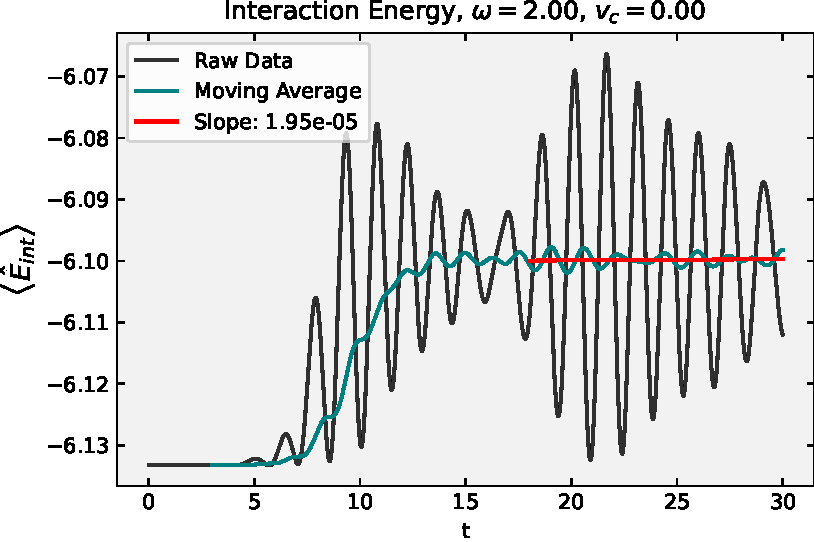
\includegraphics[width=0.49\textwidth]{graph/potential_energy/Epot_w2_vc0.pdf}
    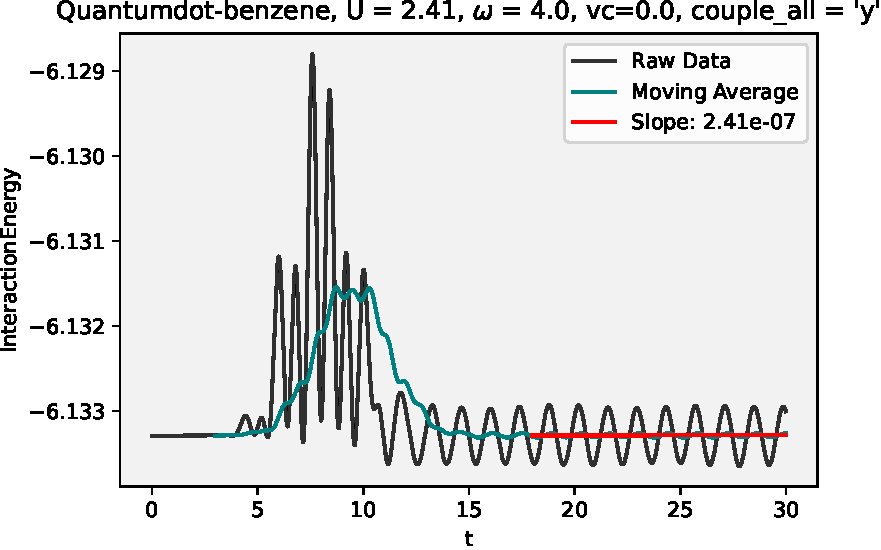
\includegraphics[width=0.49\textwidth]{graph/potential_energy/Epot_w4_vc0.pdf}
    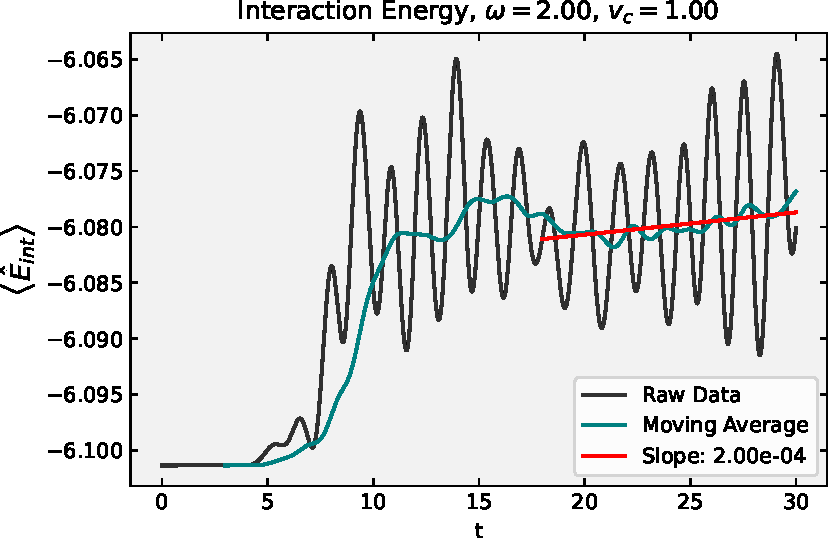
\includegraphics[width=0.49\textwidth]{graph/potential_energy/Epot_w2_vc1.pdf}
    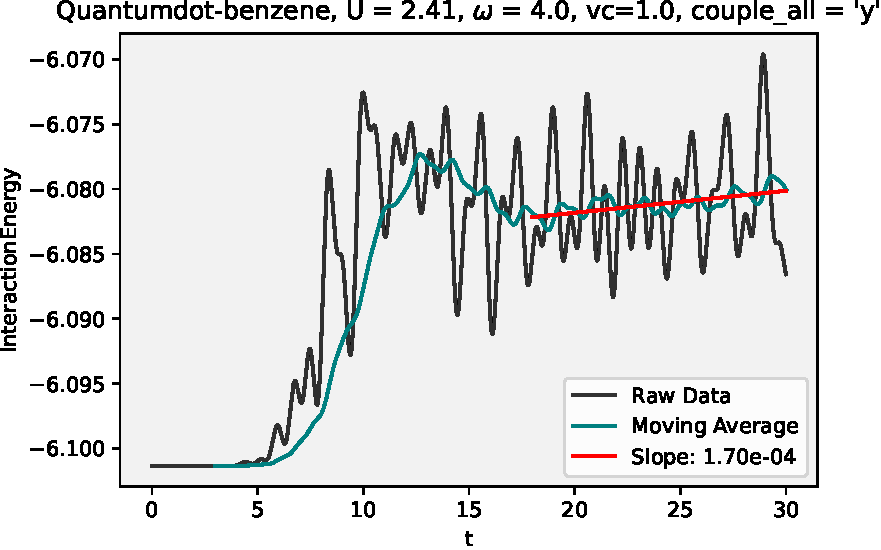
\includegraphics[width=0.49\textwidth]{graph/potential_energy/Epot_w4_vc1.pdf}
    \caption{Interaction energy of coupled system after excitation with light pulse. Shown with strong and without coupling between the QD and benzene.}
    \label{fig:interaction_energy_omega}
\end{figure}

\subsection{Occupation number changes per site over time}
Even though we can not study the interaction energy on each site individually, we can look at the occupation numbers $\braket{\hat{n}_i}$ of each site and how they evolve over time.
\medskip

In Fig. \ref{fig:occupation_vc_00} we see that for our system, which initially has $1$ electron on each site, the electrons oscillate between sites $0$ and $3$ periodically. For $\omega=4.00$ this oscillation lasts only as long as the pulse duration, but for $\omega=2.00$ it persists as energy was transferred from the pulse to the system. This is consistent with what was observed in Fig. \ref{fig:interaction_energy_omega}. Sites $1, 2$ lie perpendicular to the pulse direction (in Fig \ref{fig:occupation_vc_00} from the top right to the bottom left) and thus do not undergo any electron transfers \color{red}(Is this the only reason? Or is some symmetry argument needed as well?)\color{black}.


\begin{figure}[!hbt]
    \centering
    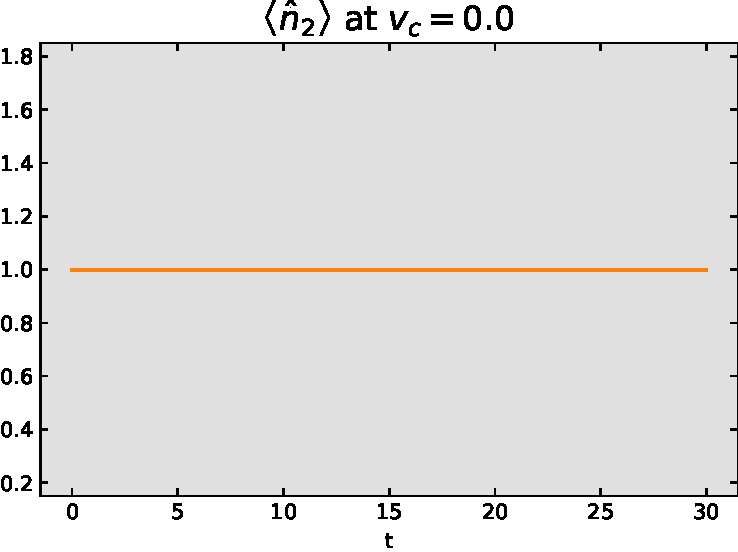
\includegraphics[width=0.35\textwidth]{graph/occupation/occupation_site_2_vc_00.pdf}
    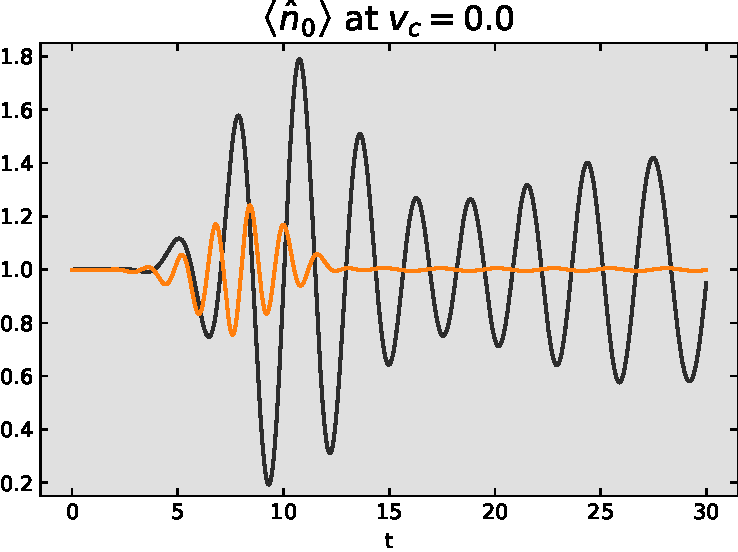
\includegraphics[width=0.35\textwidth]{graph/occupation/occupation_site_0_vc_00.pdf}
    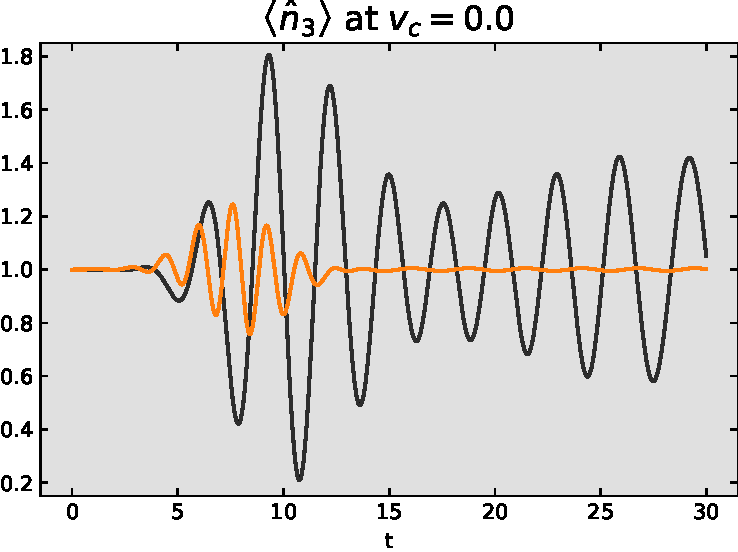
\includegraphics[width=0.35\textwidth]{graph/occupation/occupation_site_3_vc_00.pdf}
    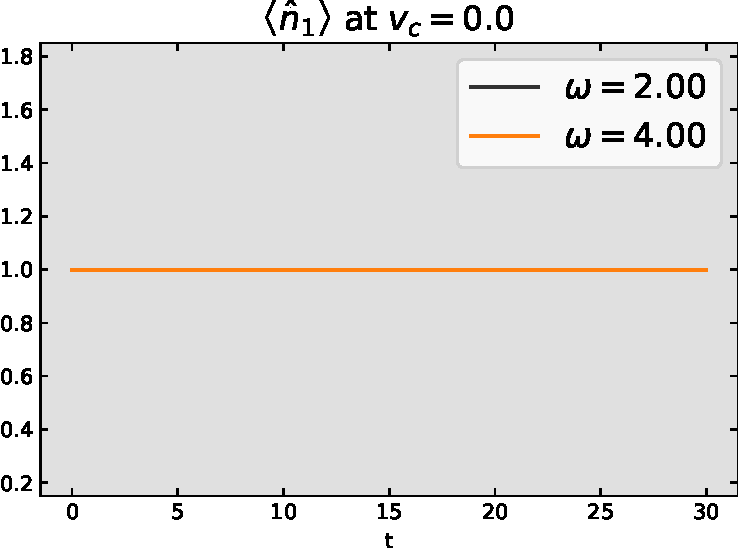
\includegraphics[width=0.35\textwidth]{graph/occupation/occupation_site_1_vc_00.pdf}
    \caption{Occupation numbers of QD sites as a function of time, at two different light pulse frequencies. Because $v_c=0$ and the benzene ring does not directly interact with the light pulse, all the occupation numbers of the benzene sites remain constant at $1$ and thus are not shown in this figure.}
    \label{fig:occupation_vc_00}
\end{figure}

\begin{figure}[!hbt]
    \begin{minipage}[b]{.49\textwidth}
                \centering
                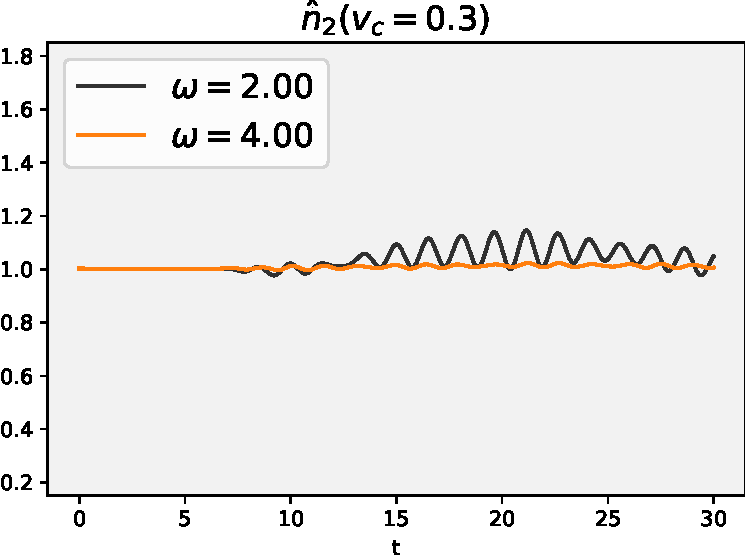
\includegraphics[trim=0 0 0 -4, clip, width=0.49\textwidth]{graph/occupation/occupation_site_2_vc_03.pdf}
                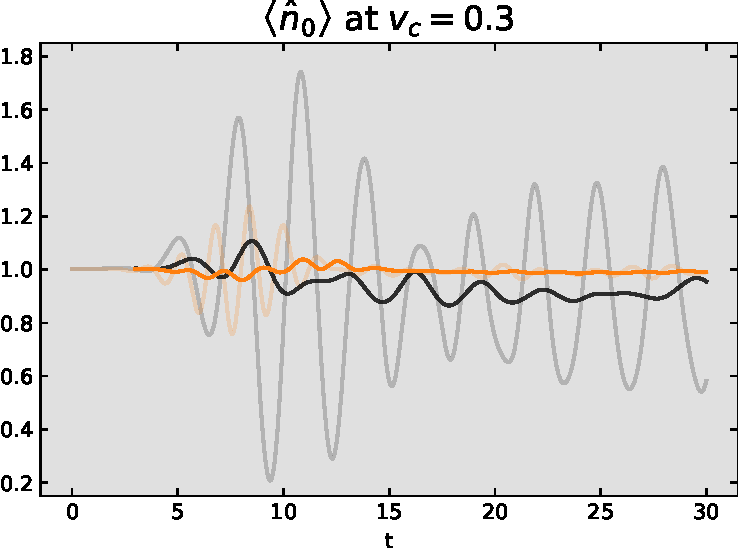
\includegraphics[trim=0 0 0 -4, clip, width=0.49\textwidth]{graph/occupation/occupation_site_0_vc_03.pdf}
                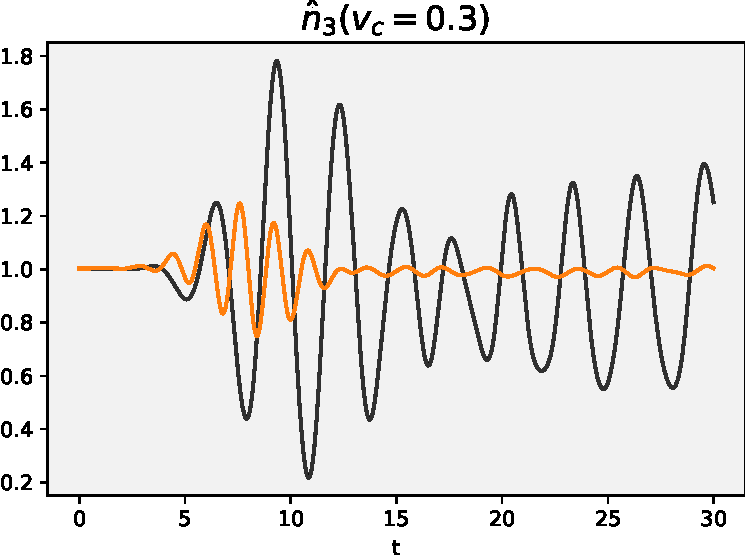
\includegraphics[trim=0 0 0 -4, clip, width=0.49\textwidth]{graph/occupation/occupation_site_3_vc_03.pdf}
                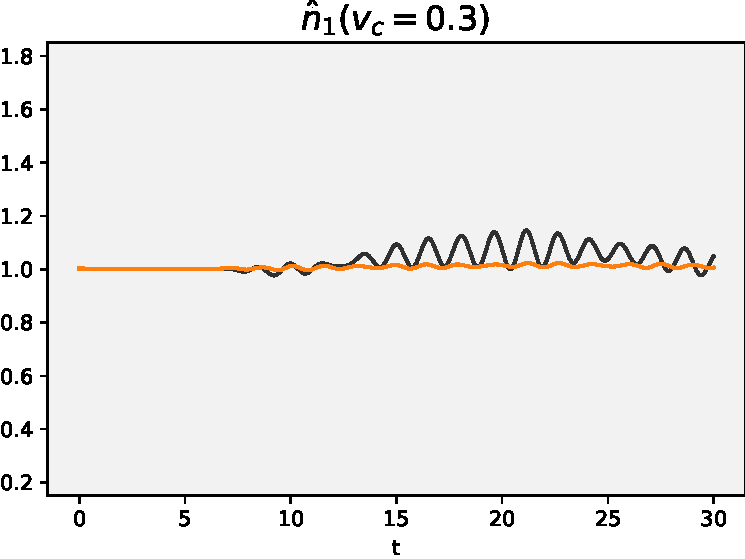
\includegraphics[trim=0 0 0 -4, clip, width=0.49\textwidth]{graph/occupation/occupation_site_1_vc_03.pdf}
                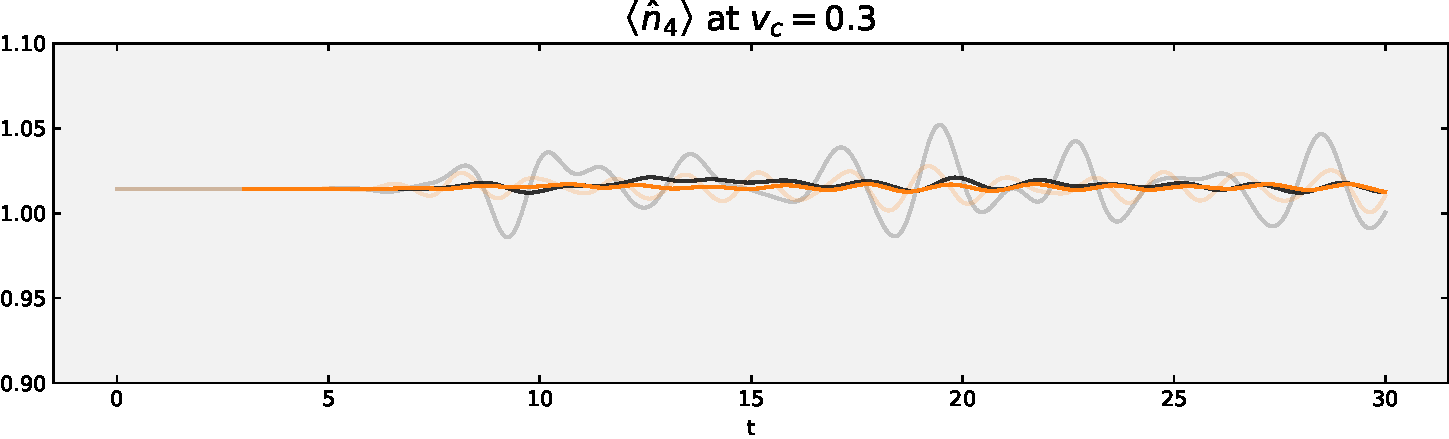
\includegraphics[trim=0 0 0 -4, clip, width=1.00\textwidth]{graph/occupation/occupation_site_4_vc_03.pdf}
                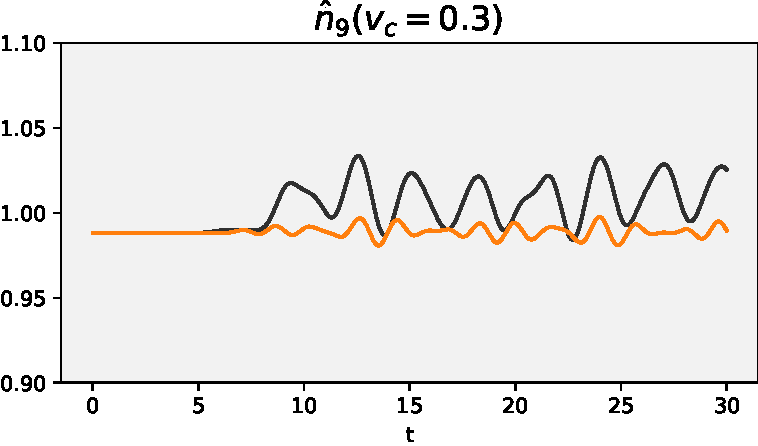
\includegraphics[trim=0 0 0 -4, clip, width=0.49\textwidth]{graph/occupation/occupation_site_9_vc_03.pdf}
                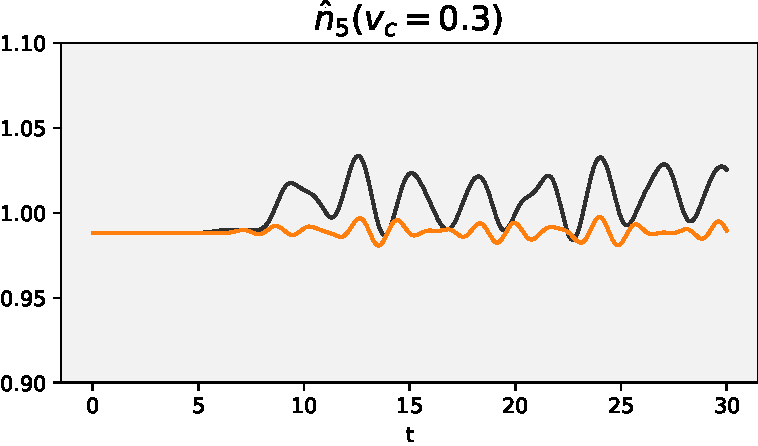
\includegraphics[trim=0 0 0 -4, clip, width=0.49\textwidth]{graph/occupation/occupation_site_5_vc_03.pdf}
                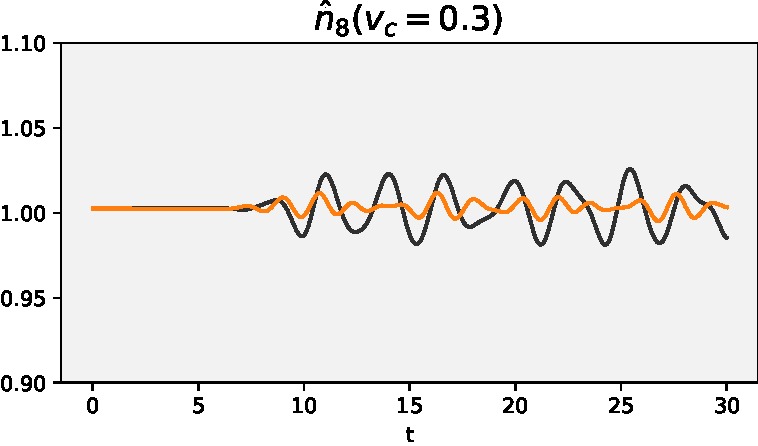
\includegraphics[trim=0 0 0 -4, clip, width=0.49\textwidth]{graph/occupation/occupation_site_8_vc_03.pdf}
                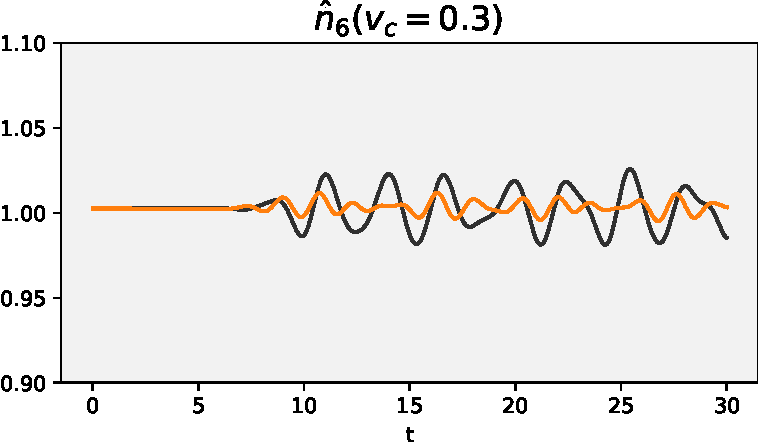
\includegraphics[trim=0 0 0 -4, clip, width=0.49\textwidth]{graph/occupation/occupation_site_6_vc_03.pdf}
                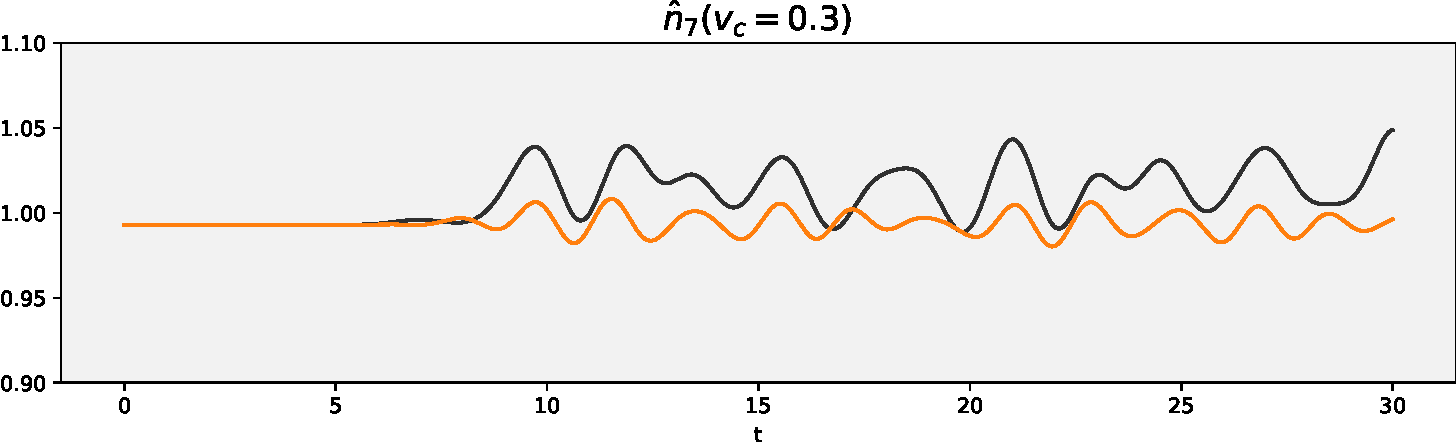
\includegraphics[trim=0 0 0 -4, clip, width=1.00\textwidth]{graph/occupation/occupation_site_7_vc_03.pdf}
       \caption{Expectation of occupation numbers for the coupled system at $v_c = 0.3$}
        \label{fig:occupation_vc_03}
    \end{minipage}
    \hfill
    \begin{minipage}[b]{.49\textwidth}
                \centering
                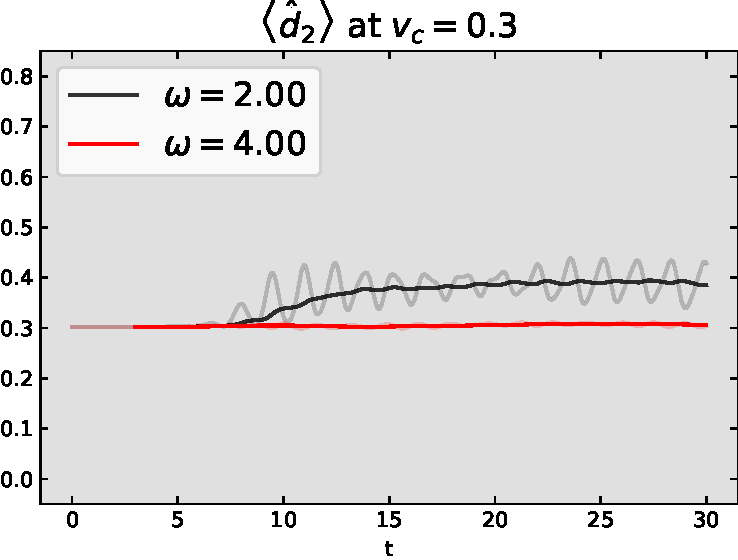
\includegraphics[width=0.49\textwidth]{graph/double_occupation/double_occupation_vc_03_site_2.pdf}
                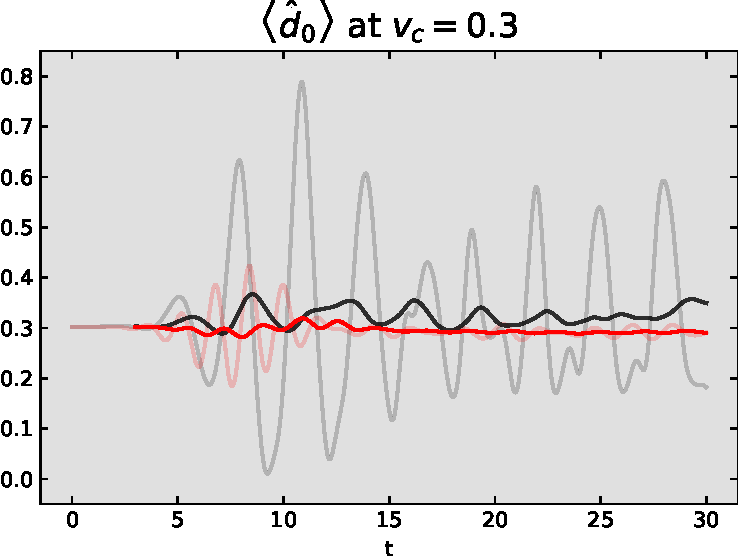
\includegraphics[width=0.49\textwidth]{graph/double_occupation/double_occupation_vc_03_site_0.pdf}
                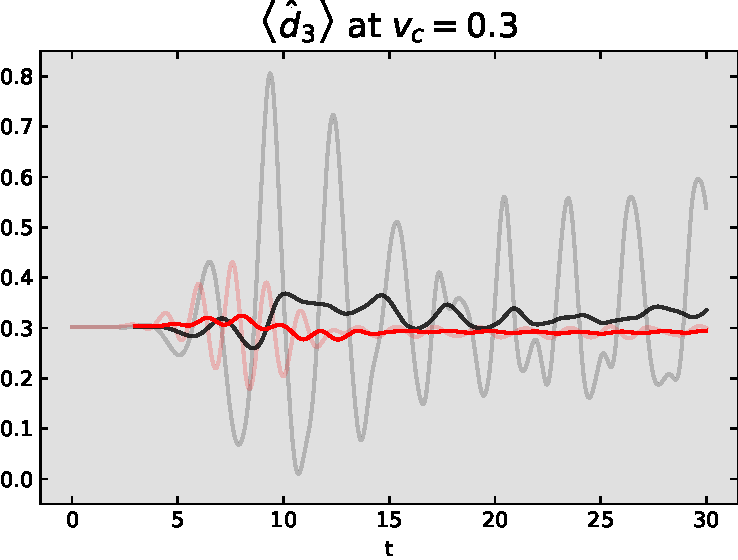
\includegraphics[width=0.49\textwidth]{graph/double_occupation/double_occupation_vc_03_site_3.pdf}
                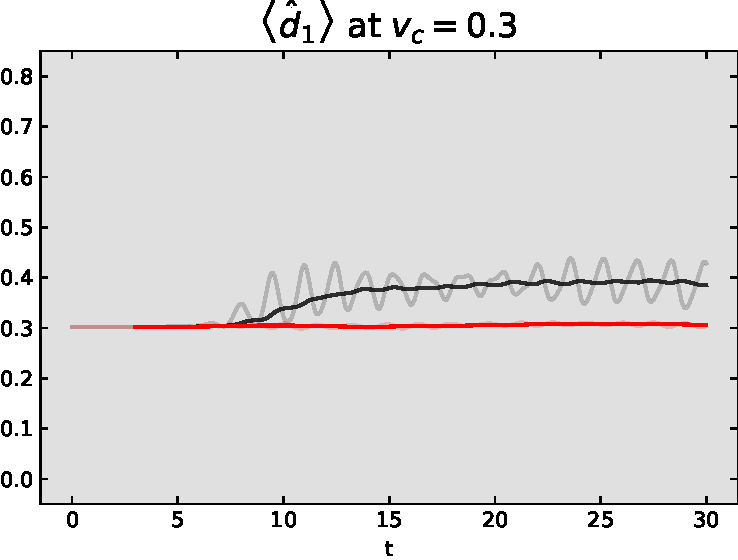
\includegraphics[width=0.49\textwidth]{graph/double_occupation/double_occupation_vc_03_site_1.pdf}
                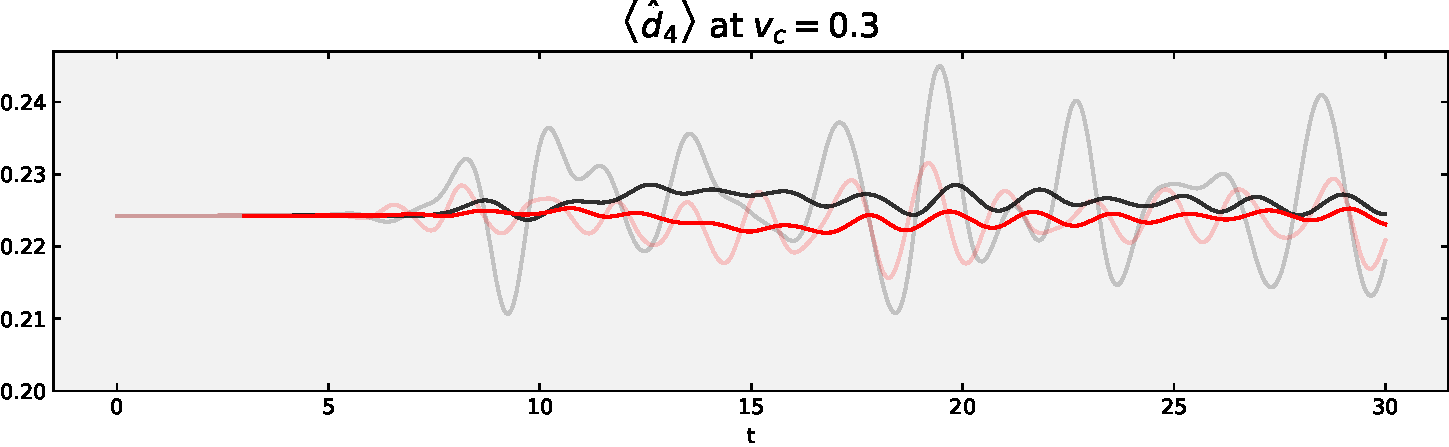
\includegraphics[width=1.00\textwidth]{graph/double_occupation/double_occupation_vc_03_site_4.pdf}
                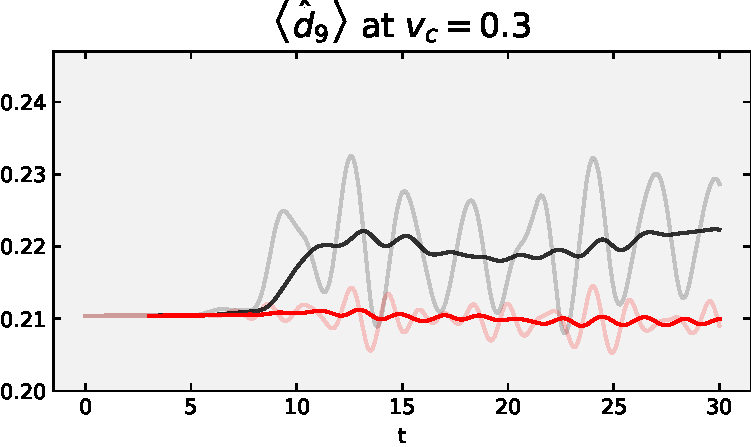
\includegraphics[width=0.49\textwidth]{graph/double_occupation/double_occupation_vc_03_site_9.pdf}
                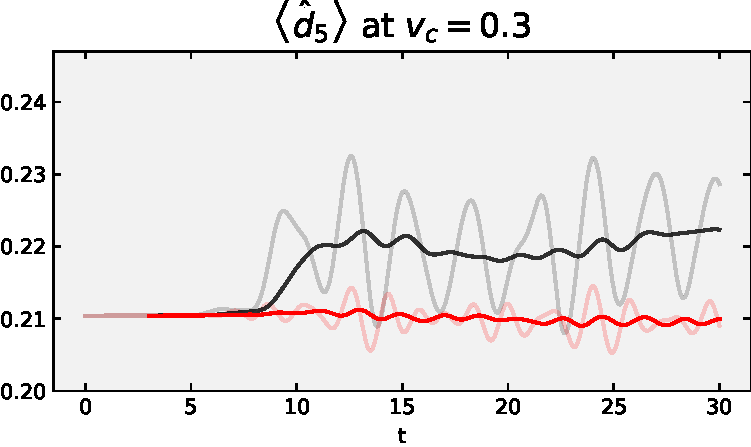
\includegraphics[width=0.49\textwidth]{graph/double_occupation/double_occupation_vc_03_site_5.pdf}
                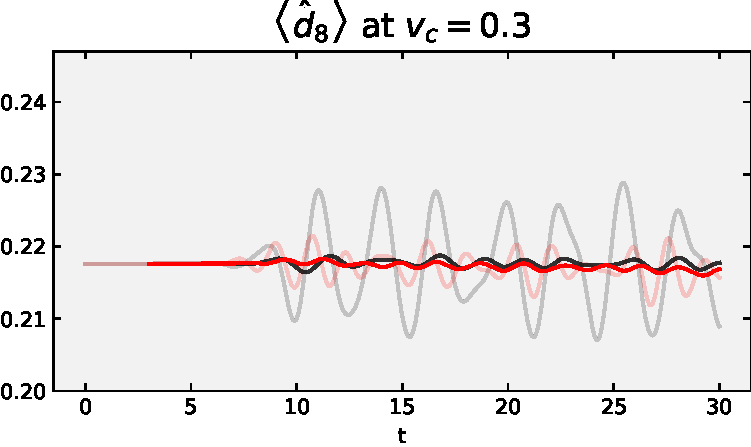
\includegraphics[width=0.49\textwidth]{graph/double_occupation/double_occupation_vc_03_site_8.pdf}
                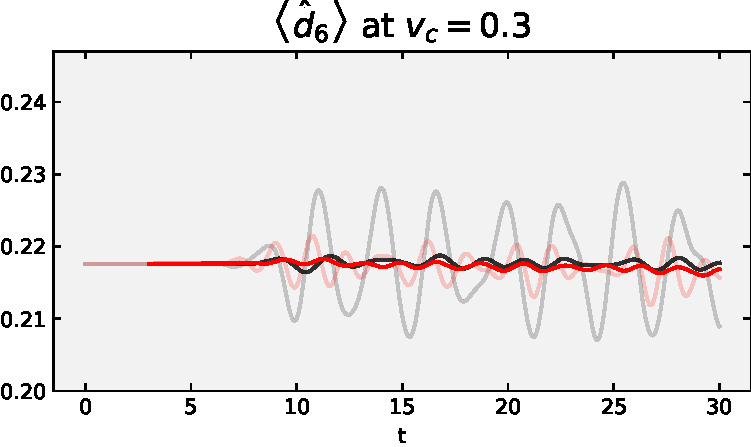
\includegraphics[width=0.49\textwidth]{graph/double_occupation/double_occupation_vc_03_site_6.pdf}
                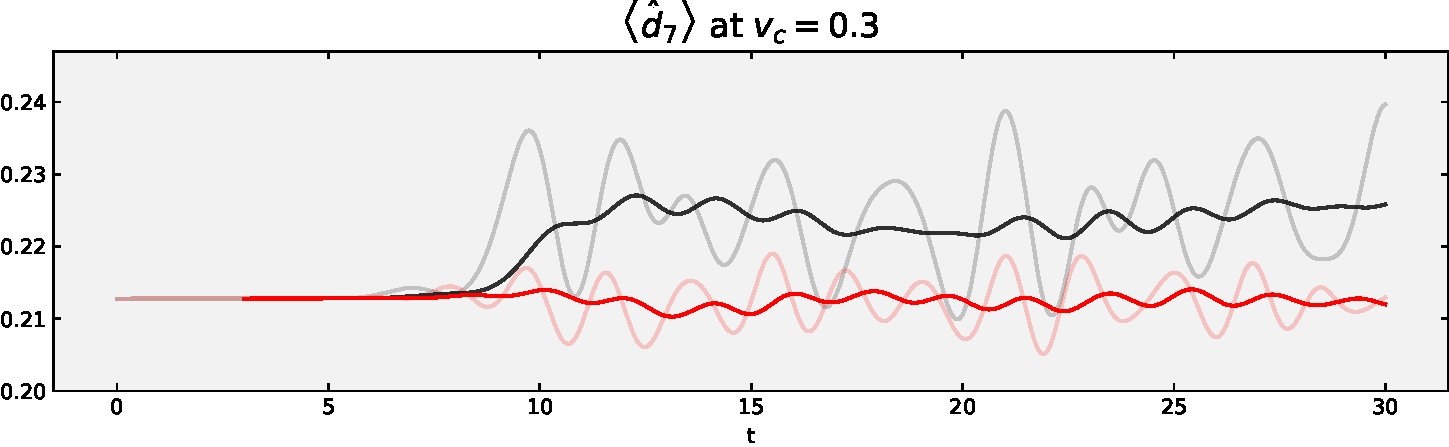
\includegraphics[width=1.00\textwidth]{graph/double_occupation/double_occupation_vc_03_site_7.pdf}
        \caption{Expectation of double occupation numbers for the coupled system at $v_c = 0.3$}
        \label{fig:double_occupation_vc_03}
    \end{minipage}
\end{figure}


\begin{figure}[!hbt]
    \begin{minipage}[b]{.49\textwidth}
                \centering
                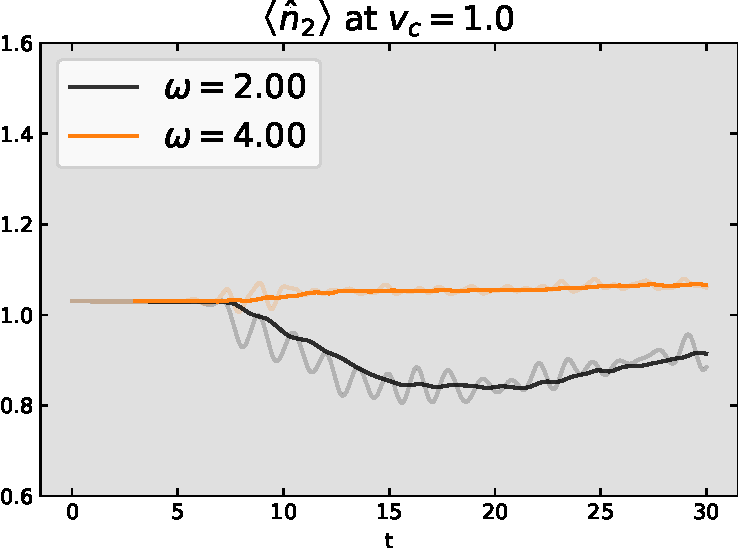
\includegraphics[trim=0 0 0 -4, clip, width=0.49\textwidth]{graph/occupation/occupation_site_2_vc_10.pdf}
                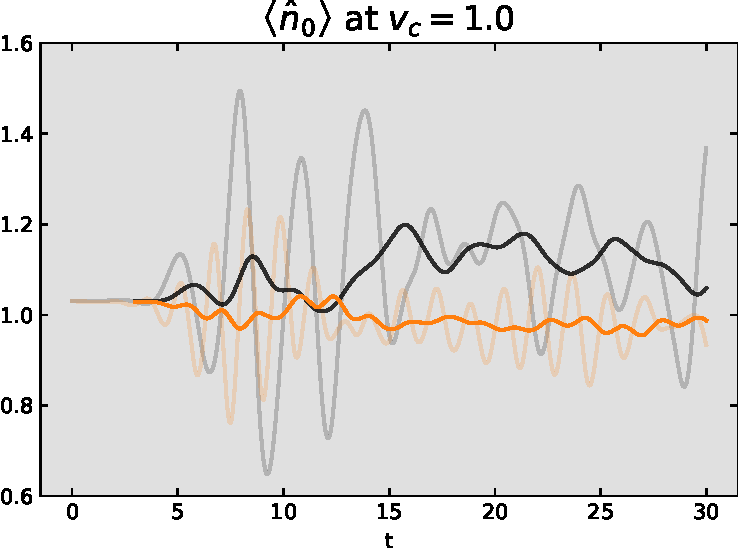
\includegraphics[trim=0 0 0 -4, clip, width=0.49\textwidth]{graph/occupation/occupation_site_0_vc_10.pdf}
                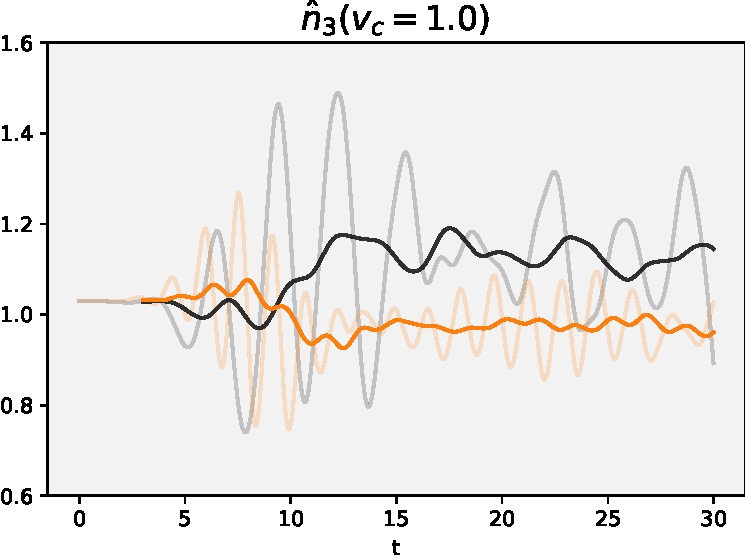
\includegraphics[trim=0 0 0 -4, clip, width=0.49\textwidth]{graph/occupation/occupation_site_3_vc_10.pdf}
                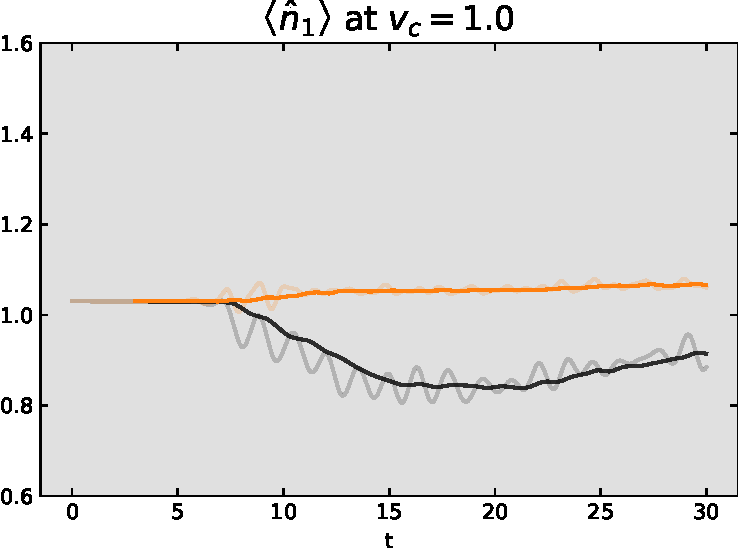
\includegraphics[trim=0 0 0 -4, clip, width=0.49\textwidth]{graph/occupation/occupation_site_1_vc_10.pdf}
                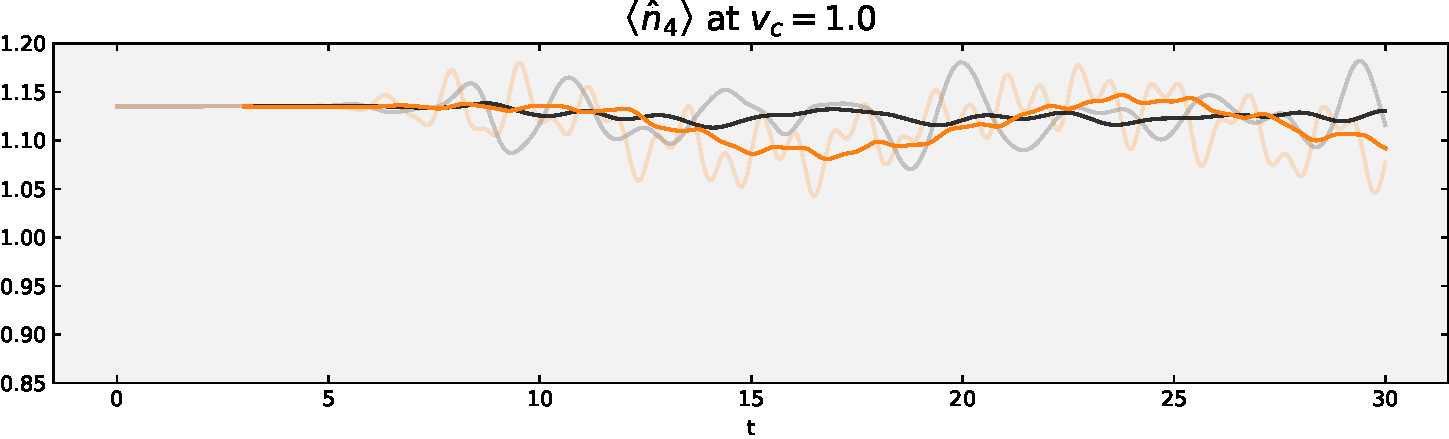
\includegraphics[trim=0 0 0 -4, clip, width=1.00\textwidth]{graph/occupation/occupation_site_4_vc_10.pdf}
                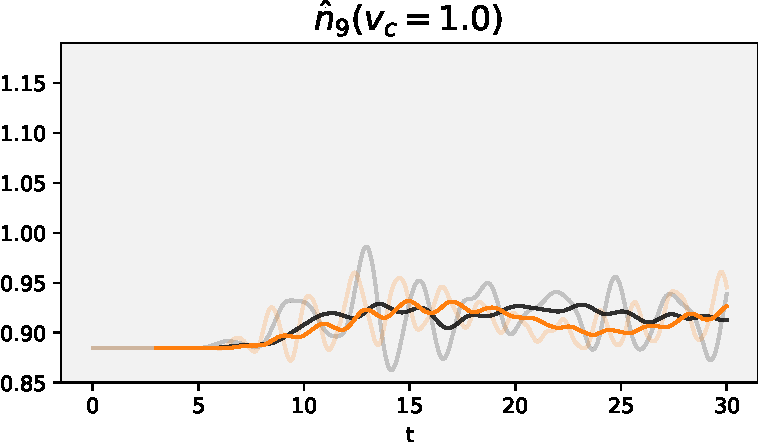
\includegraphics[trim=0 0 0 -4, clip, width=0.49\textwidth]{graph/occupation/occupation_site_9_vc_10.pdf}
                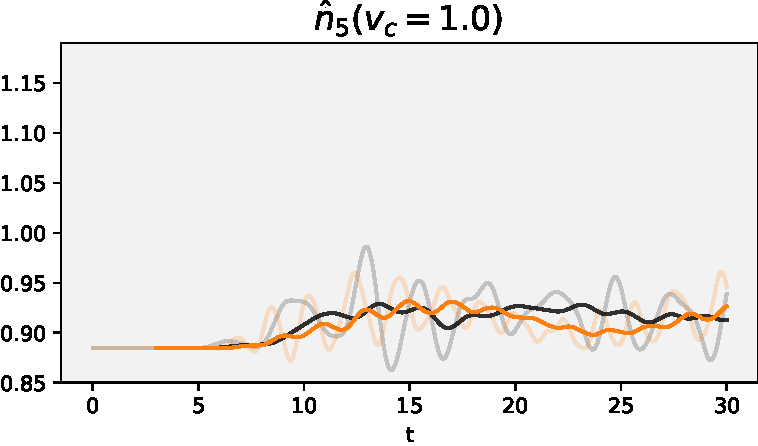
\includegraphics[trim=0 0 0 -4, clip, width=0.49\textwidth]{graph/occupation/occupation_site_5_vc_10.pdf}
                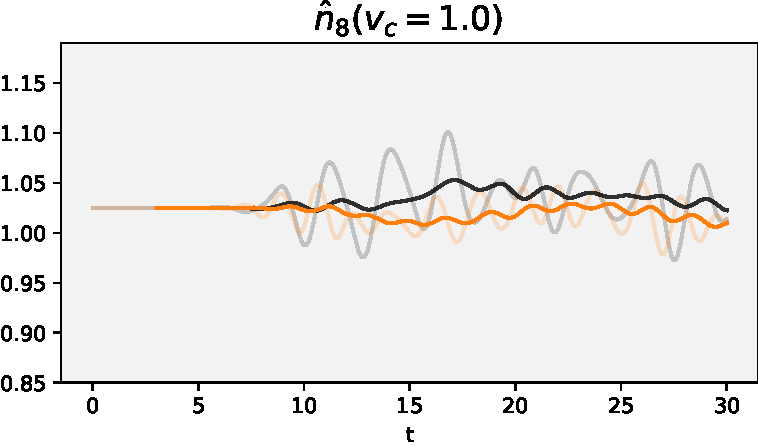
\includegraphics[trim=0 0 0 -4, clip, width=0.49\textwidth]{graph/occupation/occupation_site_8_vc_10.pdf}
                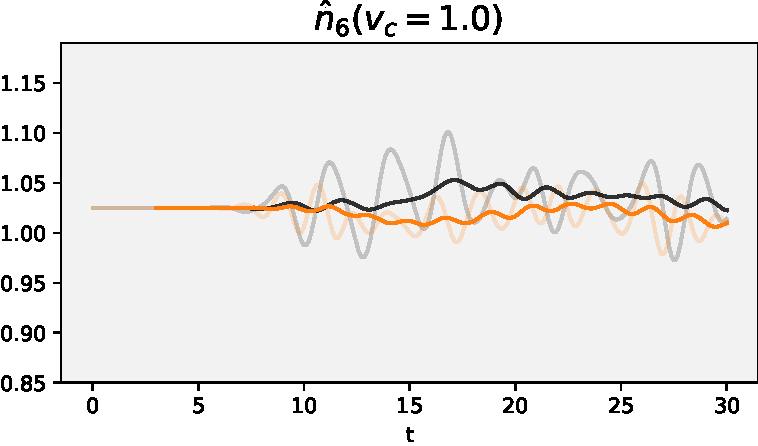
\includegraphics[trim=0 0 0 -4, clip, width=0.49\textwidth]{graph/occupation/occupation_site_6_vc_10.pdf}
                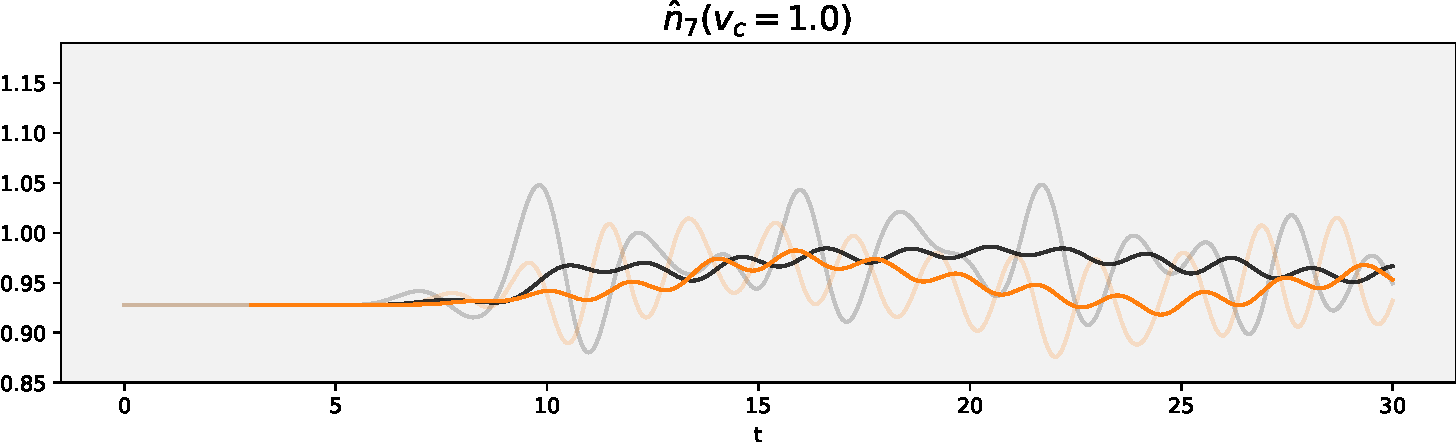
\includegraphics[trim=0 0 0 -4, clip, width=1.00\textwidth]{graph/occupation/occupation_site_7_vc_10.pdf}
       \caption{Expectation of occupation numbers for the coupled system at $v_c = 1.0$}
        \label{fig:occupation_vc_10}
    \end{minipage}
    \hfill
    \begin{minipage}[b]{.49\textwidth}
                \centering
                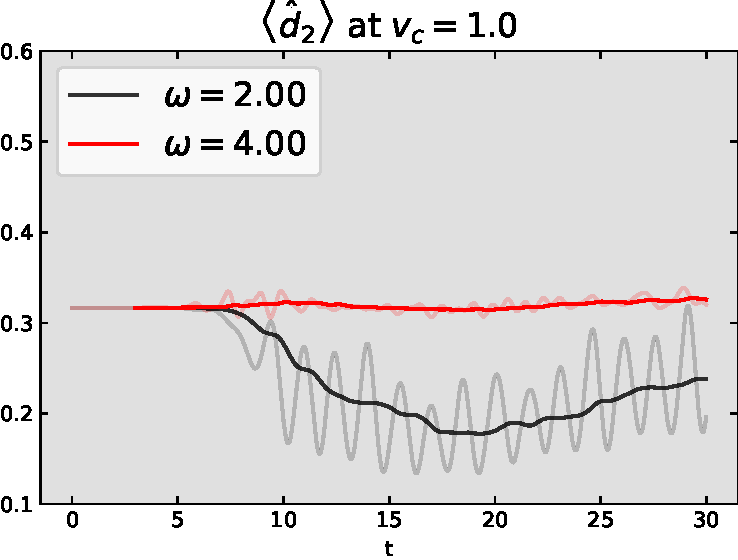
\includegraphics[width=0.49\textwidth]{graph/double_occupation/double_occupation_vc_10_site_2.pdf}
                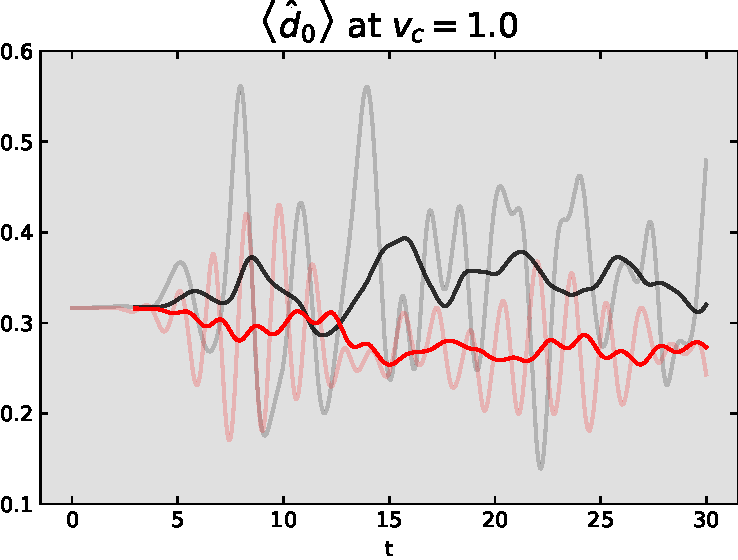
\includegraphics[width=0.49\textwidth]{graph/double_occupation/double_occupation_vc_10_site_0.pdf}
                \includegraphics[width=0.49\textwidth]{graph/double_occupation/double_occupation_vc_10_site_3.pdf}
                \includegraphics[width=0.49\textwidth]{graph/double_occupation/double_occupation_vc_10_site_1.pdf}
                \includegraphics[width=1.00\textwidth]{graph/double_occupation/double_occupation_vc_10_site_4.pdf}
                \includegraphics[width=0.49\textwidth]{graph/double_occupation/double_occupation_vc_10_site_9.pdf}
                \includegraphics[width=0.49\textwidth]{graph/double_occupation/double_occupation_vc_10_site_5.pdf}
                \includegraphics[width=0.49\textwidth]{graph/double_occupation/double_occupation_vc_10_site_8.pdf}
                \includegraphics[width=0.49\textwidth]{graph/double_occupation/double_occupation_vc_10_site_6.pdf}
                \includegraphics[width=1.00\textwidth]{graph/double_occupation/double_occupation_vc_10_site_7.pdf}
       \caption{Expectation of double occupation numbers for the coupled system at $v_c = 1.0$}
        \label{fig:double_occupatino_vc_10}
    \end{minipage}
\end{figure}

\subsection{Electron transfer between QD and benzene}
If we take the occupation number data from the previous section, and calculate the sums of occupation number expectation values on all QD and on all Benzene sites, we can observe the net electron transfer between the two coupled systems.

\begin{figure}[!hbt]
    \centering
    \includegraphics[width=0.6\textwidth]{graph/occupation/occupation_w2_03_sum.pdf}
    \caption{Caption}
    \label{fig:occupation_sum_w_2_vc_03}
\end{figure}

\begin{figure}[!hbt]
    \centering
    \includegraphics[width=0.49\textwidth]{graph/occupation/occupation_w2_Benz_sum_vcsweep.pdf}
    \includegraphics[width=0.49\textwidth]{graph/occupation/occupation_w4_Benz_sum_vcsweep.pdf}
    \caption{Caption}
    \label{fig:occupation_qd_benzene_sum_vc_03}
\end{figure}